Nesse capítulo, serão apresentados os resultados obtidos utilizando o método multiescala para solução dos sistemas lineares decorrentes do operador apresentado no Capítulo \ref{ch:modelagem}. Os resultados são apresentados na seguinte ordem: resultados em casos que a solução analítica é conhecida, visualização das soluções do espaço grosseiro, comparação entre pré-condicionador aditivo e multiplicativo, comparações do pré-condicionador multiescala, multigrid e ILU e estudo do número de iterações do solver linear com variação da tolerância do solver grosso.

\section{Soluções Analíticas}

Inicialmente, é necessário atestar que o código de elementos finitos está resolvendo corretamente o operador descrito em \eqref{eq:edp_geomec}. Para tanto, foi montado um teste semelhante ao proposto em \cite{irina}, que consiste em resolver o problema que possui como solução analítica apresentada em \eqref{eq:irinasol} em um domínio  $L \times W$.


\begin{equation} \label{eq:irinasol}
  \begin{aligned}
  u_x = 10^{-5} sen(\frac{\pi x}{L}) sen(\frac{\pi y}{W})  \\
  u_y = 10^{-5} sen(\frac{\pi (L-x)}{L}) sen(\frac{\pi x}{W})
  \end{aligned}
\end{equation}

Dada a solução, é possível calcular o lado direito correspondente a essa solução aplicando o lado esquerdo de \eqref{eq:edp_geomec} e obtendo a função $f: R^2 \rightarrow R^2$ apresentada em \eqref{eq:irinald}. 

\begin{equation} \label{eq:irinald}
f(x, y) = 
\left[\begin{matrix}\frac{E \left(- 2 v + \pi^{2} y \left(v - 1\right) \left(y - 2\right) + 1\right) \sin{\left (\pi x \right )}}{\left(v + 1\right) \left(2 v - 1\right)} \\ \frac{\pi E \left(y - 1\right) \cos{\left (\pi x \right )}}{\left(v + 1\right) \left(2 v - 1\right)}\end{matrix}\right]
\end{equation}

Dessa forma, as equações que representam o problema resolvido são apresentadas em \eqref{eq:irinaproblem}. 

\begin{equation}\label{eq:irinaproblem}
    \begin{aligned}
        S^T C S u = f(x, y), \\
        u(x,y) = [0, 0]^T, \text{ em } \Gamma ,\\
        L = W = 10.
    \end{aligned}
\end{equation}

O erro entre a solução calculada pelo método dos elementos finitos pode então ser comparada
com a solução analítica através do erro relativo mostrado em \eqref{eq:erroAnalitico}.

\begin{equation} \label{eq:erroAnalitico}
    \epsilon_{\infty} =\frac{|u_{fem} - u_{ref}|_{\infty}}{|u_{ref}|_{\infty}}
\end{equation}
onde $u_{ref} = [u_x(x_0, y_0), u_y(x_1, y_1), ..., u_x(x_{n_n}, y_{n_n})]^T$ e $u_{fem}$ é a solução obtida com o método dos elementos finitos. A variação do erro com o tamanho da discretização do domínio é mostrado na Figura  \ref{fig:SecondErrorTest} onde no eixo x o logaritmo do tamanho de cada elemento ($\Delta x$) de cada elemento e no eixo y o logaritmo de $\epsilon_{\infty}$. Também como referência é mostrada uma reta de coeficiente angular $2$ para comprovar o decaimento quadrático do erro.


\begin{figure}[h]
\center
\subfigure[ ]{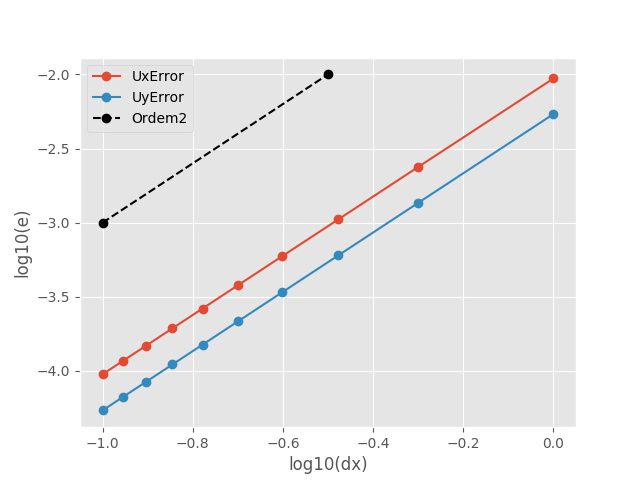
\includegraphics[width=0.45\textwidth]{chap08/figs/SecondErrorTest.png}\label{fig:SecondErrorTest}}
\qquad
\subfigure[ ]{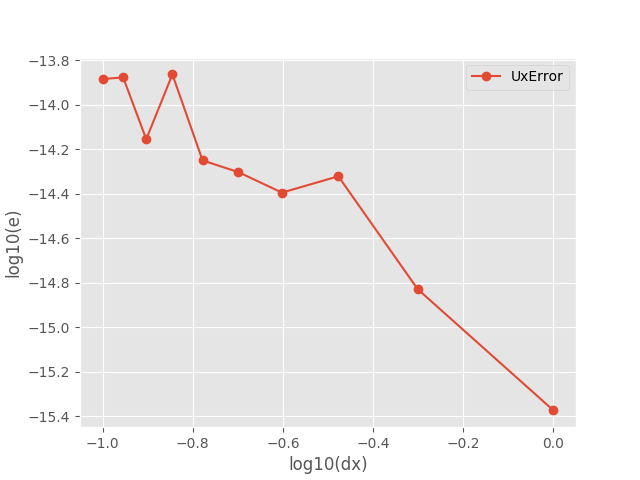
\includegraphics[width=0.45\textwidth]{chap08/figs/SecondErrorTestSimpleShear.png}    \label{fig:SecondErrorTestSimpleShear}}
\caption{Gráficos do logaritmo do erro \eqref{eq:erroAnalitico} em função do logaritmo do tamanho $\Delta x$ dos elementos do grid.}
\end{figure}
    
    
Um segundo caso com resultado analítico é o cisalhamento puro (Simple Shear). Nesse caso, o problema é definido na forma apresentada em \eqref{eq:simpleshear}  e solução é dada por $u(x,y) = [y, 0]^T$. Como a solução é um polinômio do primeiro grau, essa pode ser representada exatamente no espaço gerado pelas funções de base bilineares e, então, os erros de truncamento, nesse caso, não existem, restando apenas  erros de arredondamento. \suge{Talvez seja o caso de definir, nos capítulos anteriores, o que são os \textit{erros de truncamento e de arredondamento}, apenas para o texto ser autocontido}

\begin{equation}\label{eq:simpleshear}
    \begin{aligned}
        S^T C S u = 0, \\
        u(x,y) = [10^{-6}, 0]^T, \text{ em } \{x, y \in \Gamma | y \neq 1\} ,\\
        u(x,y) = [10^{-6}y, 0]^T, \text{ em } \{x, y \in \Gamma | x = 0 \text{ ou } x = 1\}, \\
        u(x,y) = [0, 0]^T, \text{ em } y=0.
    \end{aligned}
\end{equation}

A variação do erro com o tamanho da malha é apresentado na Figura \ref{fig:SecondErrorTestSimpleShear} e pode-se observar que nesse caso o maior erro relativo é menor que $10^{-12}$ que é bem menor que o do caso anterior, por conta do erro de truncamento ser zero, e também não decai com o tamanho da malha.

Atestado o bom funcionamento do método dos elementos finitos, os resultados das próximas seções irão tomar como referência as soluções no grid fino, já que soluções analíticas não estão disponíveis.


\section{Modelos de simulação utilizados}

 A Tabela \ref{tab:descricaoModelos} apresenta os tamanhos dos modelos utilizados neste trabalho. Cinco modelos foram selecionados onde dois deles são de modelos de campos reais. Os casos A e B são baseados nos casos sintéticos apresentados em \cite{casteletto} e \cite{irina}, nesses casos foram utilizados uma compressibilidade vertical uniaxial $c_M$ desenvolvida em \cite{correlacaoE} apresentada em \eqref{eq:correlacaoCm}, onde $c_M$ e $\sigma_y^\prime$ são expressas em [bar$^{-1}$] e [bar] e  $\sigma_y^\prime$ representa a tensão vertical efetiva, e a tensão efetiva na rocha é calculada através de  \eqref{eq:correlacaoTensao} que considera um gradiente de pressão de 0.1 bar/m e coeficiente de Biot igual a um.

\begin{table}[]
    \caption{Tabela com os casos que serão apresentados os resultados. }\label{tab:descricaoModelos}
    \centering
    \begin{tabular}{ccccl}
    \cline{1-4}
    \multicolumn{1}{|c|}{\textbf{Nome}} & \multicolumn{1}{c|}{\textbf{Nx}} & \multicolumn{1}{c|}{\textbf{Ny}} & \multicolumn{1}{c|}{\textbf{Caso Real}} &  \\ \cline{1-4}
    \multicolumn{1}{|c|}{caso A}        & \multicolumn{1}{c|}{100}         & \multicolumn{1}{c|}{100}         & \multicolumn{1}{c|}{Não}                   &  \\ \cline{1-4}
    \multicolumn{1}{|c|}{caso B}        & \multicolumn{1}{c|}{320}         & \multicolumn{1}{c|}{320}         & \multicolumn{1}{c|}{Não}                   &  \\ \cline{1-4}
    \multicolumn{1}{|c|}{caso C}        & \multicolumn{1}{c|}{103}         & \multicolumn{1}{c|}{56}          & \multicolumn{1}{c|}{Não}                   &  \\ \cline{1-4}
    \multicolumn{1}{|c|}{caso D}        & \multicolumn{1}{c|}{244}         & \multicolumn{1}{c|}{71}          & \multicolumn{1}{c|}{Sim}                &  \\ \cline{1-4}
    \multicolumn{1}{|c|}{caso E}        & \multicolumn{1}{c|}{582}         & \multicolumn{1}{c|}{336}         & \multicolumn{1}{c|}{Sim}                &  \\ \cline{1-4}
    \multicolumn{1}{l}{}                & \multicolumn{1}{l}{}             & \multicolumn{1}{l}{}             & \multicolumn{1}{l}{}                    &  \\
    \multicolumn{1}{l}{}                & \multicolumn{1}{l}{}             & \multicolumn{1}{l}{}             & \multicolumn{1}{l}{}                    & 
    \end{tabular}
\end{table}


% TODO modificar tabelas para esse o padrão abaixo 

% \begin{table}[htb]
%     \caption{Tabela com os casos que serão apresentados os resultados. }\label{tab:descricaoModelos_lmc}
%     \centering
%     \begin{tabular}{@{}cccc@{}}
%     \toprule
%     \textbf{Nome}&\textbf{Nx}&\textbf{Ny}&\textbf{Caso Real}\\
%     \midrule
%     caso A &100 &100 & Não\\
%     caso B &320 &320 & Não\\
%     caso C &103 &56 & Não\\
%     caso D &244 &71 & Sim\\
%   caso E & 582 &336 & Sim\\
%     \bottomrule
%     \end{tabular}
% \end{table}
    

\begin{equation} \label{eq:correlacaoCm}
    c_M = 0.01241 |\sigma_y^\prime|^{-1.1342}
\end{equation}

\begin{equation} \label{eq:correlacaoTensao}
\sigma_y^\prime = \sigma_y + p = -0.12218|y| + 0.1 |y|
\end{equation}

Assim, o módulo de Young pode ser calculado em função apenas da profundidade substituindo os valores de \eqref{eq:correlacaoCm} e \eqref{eq:correlacaoTensao} em \eqref{eq:correlacaoYoung}. Já o coeficiente de Poisson foi considerado constante e igual a 0.2 em todo o modelo. 

\begin{equation} \label{eq:correlacaoYoung}
    E = \frac{(1-2\poisson)(1+\poisson)}{(1-\poisson)c_M}
\end{equation}

O grid utilizado é apresentado na Figura \ref{fig:gridBase10x10} com as dimensões baseadas no exemplo mostrado em \cite{casteletto}. Esse grid teve cada uma das células divididas em com 10 cortes verticais e 10 cortes horizontais igualmente espaçados para gerar o caso A e de forma análoga dividida em 32 cortes horizontais e 32 cortes verticais para gerar o caso B. A localização do reservatório aparece na Figura \ref{fig:gridBase10x10} em vermelho. Foi considerada também a depleção de 100 bar de pressão no reservatório.

\begin{figure}[!htbp]
    \centering
    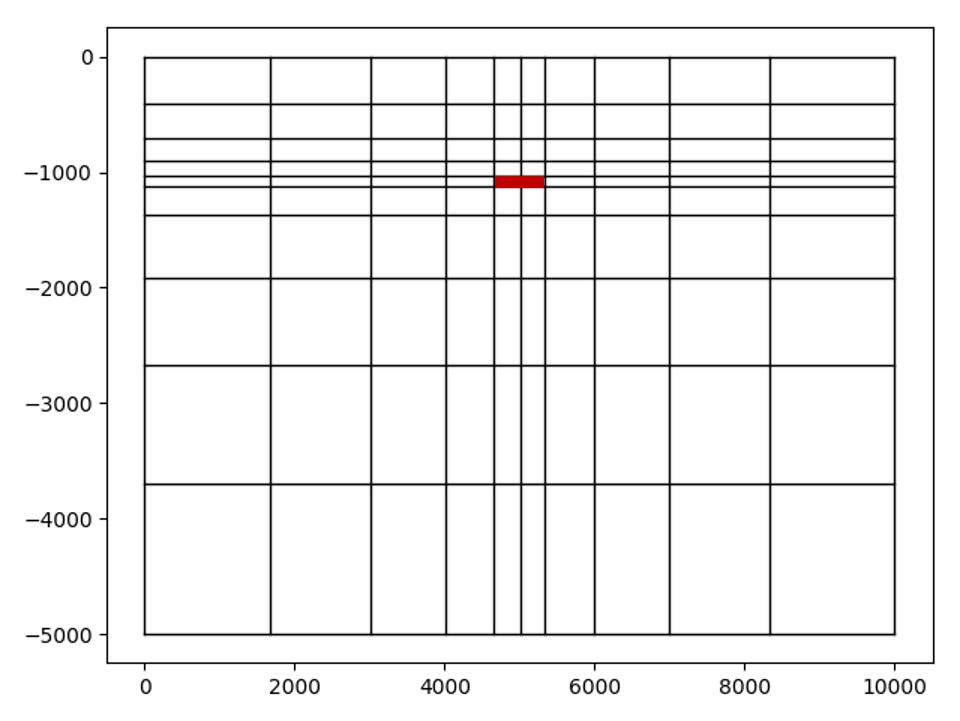
\includegraphics[height=6cm]{chap08/figs/Reservoir10x10_grid.png}
    \caption{Grid base utilizado para construção dos casos A e B.}
    \label{fig:gridBase10x10}
\end{figure}


O caso C é um caso de reservatório sintético com grid de geometria mais próxima aos reservatórios reais e,  diferentemente dos casos A e B, os valores de poisson não são constantes ao longo do domínio. A Figura \ref{fig:casoCgrid} no anexo \ref{ch:figurasReservatorios} apresenta o grid e os valores do módulo de Young e módulo de Poisson. São apresentados também no apêndice figuras dos casos D e E que tiveram as escalas omitidas por se tratarem de modelos de campos reais.


As condições de contorno utilizadas para todos os modelos são representadas na Figura \ref{fig:CondicoesContorno}, a base do modelo é considerada fixa ($u=0$), as bordas laterais tem movimento possível apenas na direção y e topo do modelo é livre de tração.

\begin{figure}[!htbp]
    \centering
    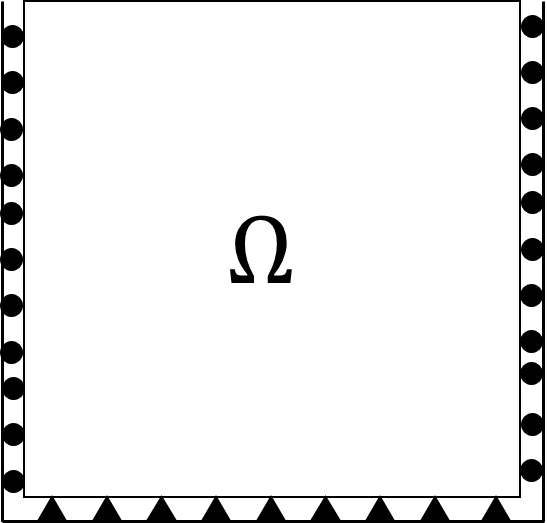
\includegraphics[height=4cm]{chap08/figs/CondicoesContorno.png}
    \caption{Esquema das condições de contorno das simulações. Borda inferior com deslocamentos nulos, bordas laterais com deslocamentos em y permitidos e borda superior livre.}
    \label{fig:CondicoesContorno}
\end{figure}


\section{Resultados Método Multiescala}

\subsection{Visualização da solução grossa}

Dada que o operador multiescala gera um operador grosso com solução que tenta reproduzir a solução do espaço fino, é possível comparar visualmente e também através do erro entre a solução fina e a solução da malha grossa. No caso, a aproximação para a solução da malha fina $u^h_{ms} = P u^H$ é utilizada nessa comparação de forma que o erro que será apresentado é mostrado em \eqref{eq:erroMS}.

\begin{equation}\label{eq:erroMS}
\epsilon_{\infty} =\frac{|u^h - P u^H|_{\infty}}{|u^h|_{\infty}}
\end{equation}


As Figuras presentes em \ref{fig:comparacaoFinoGrosso} apresentam a comparação entre a solução do grid fino e do grosso. Pode-se notar que a solução é distorcida mas mesmo assim guarda similaridades com a solução original. Para uma avaliação quantitativa é apresentada a \ref{table:erroRelativoEngrossamento}. A Figura \ref{fig:subsidence} mostra a subsidência do topo do reservatório para a solução fina e solução grossa.


\begin{table}[]
\centering

\caption{Erro relativo da solução fina em relação a grossa para diferentes níveis de engrossamento.}
\label{table:erroRelativoEngrossamento}

\begin{tabular}{|c|c|}
\hline
\textbf{Nível de Engrossamento} & \textbf{Erro Relativo} \\ \hline
8x8                             & 0.124267               \\ \hline
16x16                           & 0.190326               \\ \hline
32x32                           & 0.273388               \\ \hline
64x64                           & 0.763958               \\ \hline
\end{tabular}
\end{table}


\begin{figure}[h]
\center
\subfigure[ Solução do grid fino. À esquerda, o deslocamento em x e, à direita, o deslocamento em y]{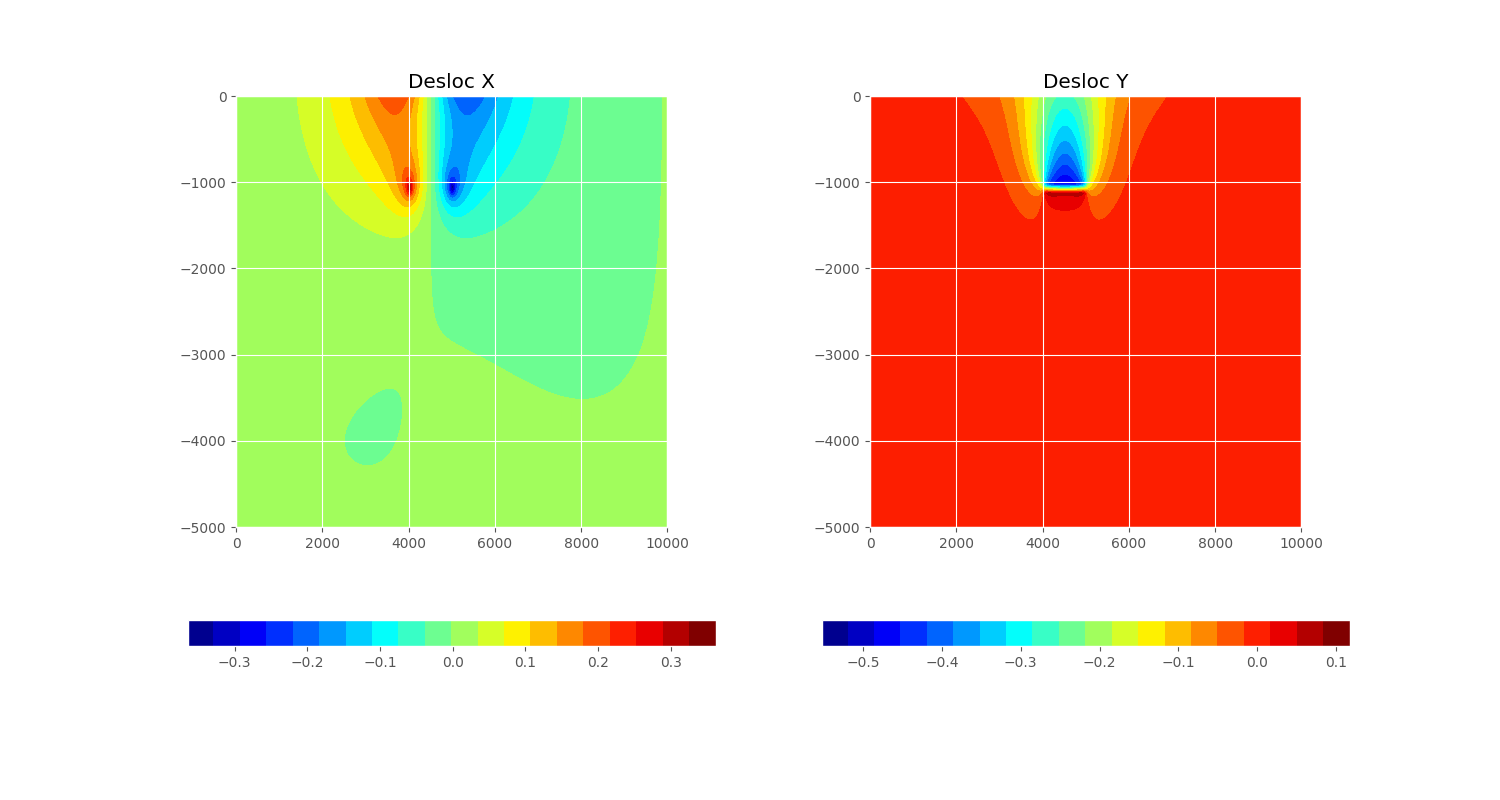
\includegraphics[width=\textwidth]{chap08/figs/Reservoir320x320_10x10_permanent.png}\label{fig:casoB_10x10_fine}}
\qquad
\subfigure[Solução do grid grosso. À esquerda, o deslocamento em x e, à direita, o deslocamento em y ]{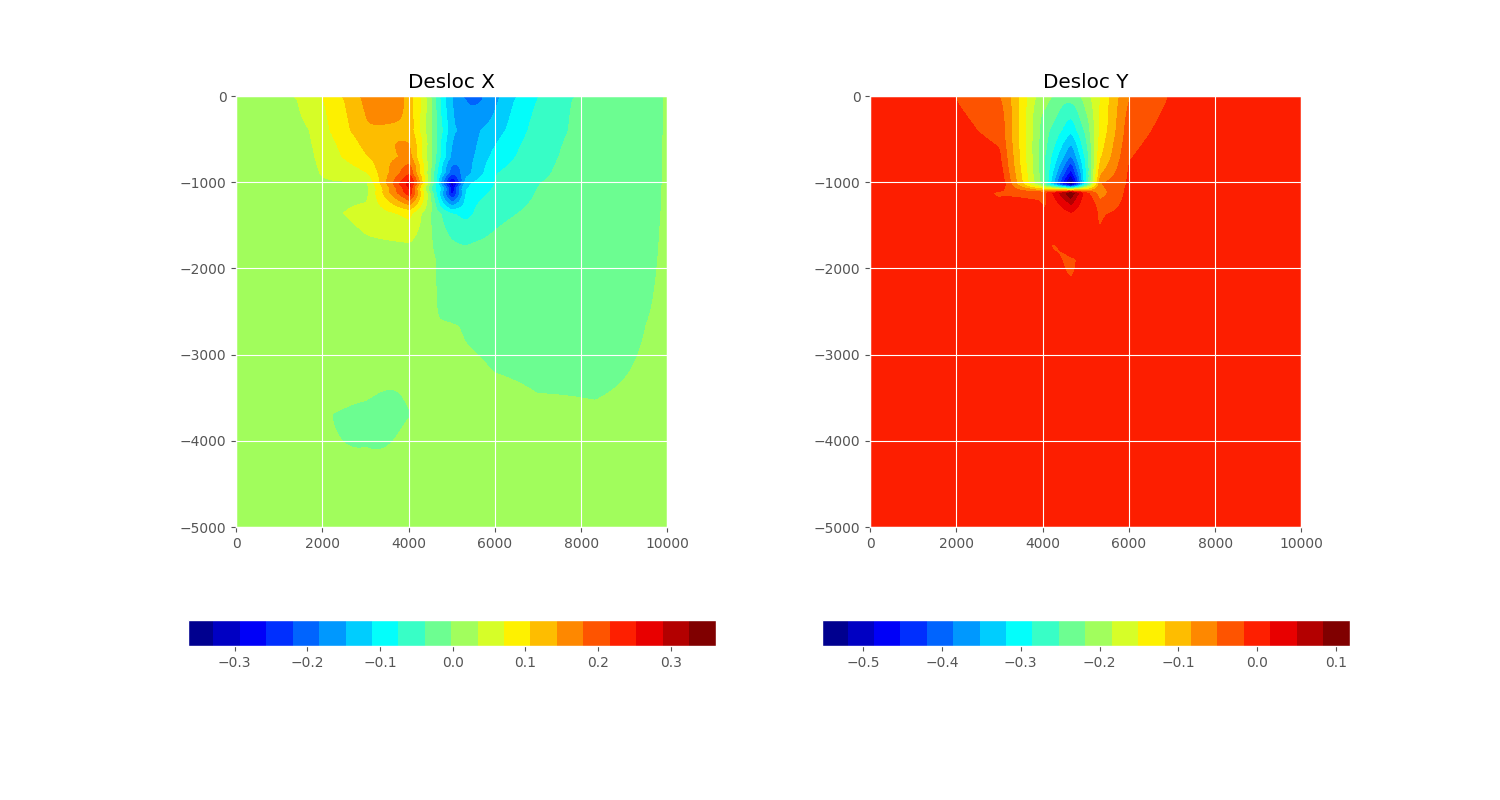
\includegraphics[width=\textwidth]{chap08/figs/Reservoir320x320_10x10_permanent_multiscale_total.png}\label{fig:casoB_10x10_fine_coarse}}
\caption{Comparação da solução do grid fino com a solução do grid grosso.  }
\label{fig:comparacaoFinoGrosso}
\end{figure}

\begin{figure}[!htbp]
\centering
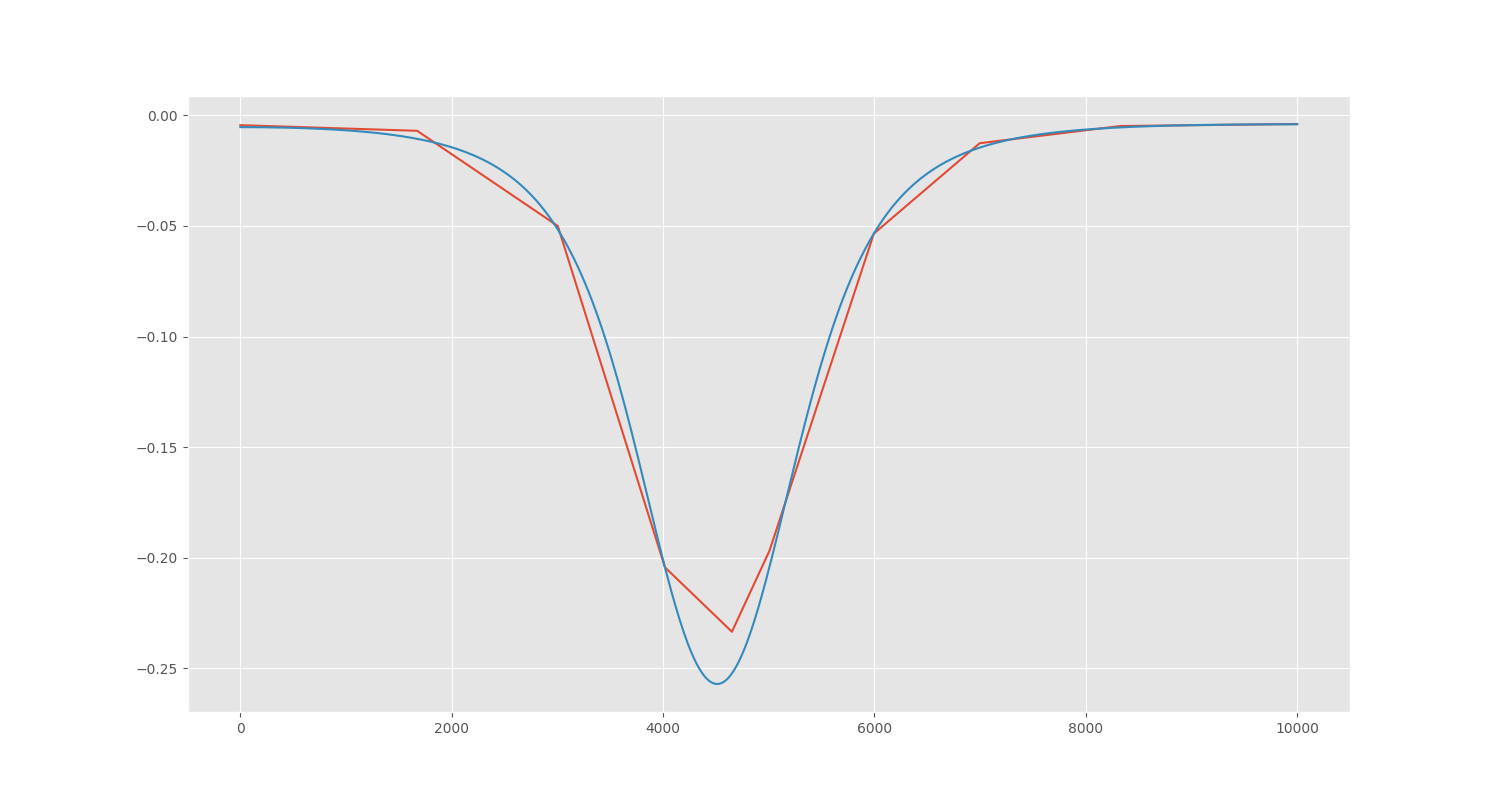
\includegraphics[width=0.8\textwidth]{chap08/figs/Reservoir320x320_10x10_subsidence_multiscale.png}
\caption{Subsidência do topo do caso B, em azul na solução do grid fino e de vermelho a solução do grid grosso. }
\label{fig:subsidence} 
\end{figure}


\subsection{Comparação entre pré-condicionadores aditivos e multiplicativos}

O trabalho \cite{casteletto} apresenta a utilização do pré-condicionador multiescala ($M_{ms}$) em conjunto com o um pré-condicionador ($M_h$) no grid fino de forma multiplicativa. 
Essa combinação visa reduzir os erros de alta frequência através do $M_h$ enquanto os erros de baixa frequência são eliminados pelo pré-condicionador multiescala. 
O acoplamento multiplicativo tem a desvantagem de precisar de uma multiplicação matriz vetor além da aplicação dos pré-condicionadores
e, portanto, o número de iterações tem que ser reduzido o suficiente para compensar todas essas operações. Um alternativa é aplicação
dos pré-condicionadores de forma aditiva, pois, nesse caso, não é necessária a multiplicação matriz vetor adicional. Outra vantagem do operador aditivo é que caso os $M_h^{-1}$ e $M_{ms}^{-1}$ sejam simétricos o pré-condicionador conjunto também é simétrico e pode ser utilizado juntamente com o gradiente conjugado com garantia de convergência.


As tabelas \ref{table:precondcasoAcomp} e \ref{table:precondcasoBcomp} mostram a quantidade de iterações e os respectivos resíduos da solução do sistema linear utilizando o pré-condicionador aditivo e o multiplicativo junto com o solver Bicgstab. Nesses testes o pré-condicionador $M_h^{-1}$ foi o ILU(0).

É importante notar que a quantidade de iterações do dois métodos é bem próxima, em casos em que até o operador aditivo é mais eficiente que o multiplicativo. Dessa forma, uma alternativa a utilizar o Bicgstab com o pré-condicionador aditivo é utilizada o Gradiente conjugados juntamente com o pré-condicionador aditivo.

\begin{table}[]
    \caption{Comparação de pré-condicionador aditivo contra multiplicativo para caso A utilizando como solver linear o método Bicgstab para diferentes níveis de engrossamento.}
    \label{table:precondcasoAcomp}
    \begin{tabular}{c|c|c|c|l|}

    \cline{2-5}
                                          & \multicolumn{4}{c|}{Pré-condicionador}                                                        \\ \cline{2-5} 
                                          & \multicolumn{2}{c|}{$\preconmult$}               & \multicolumn{2}{c|}{$\preconadd$}                \\ \hline
    \multicolumn{1}{|c|}{Elemento Grosso} & Iterações & \multicolumn{1}{c|}{Resíduo}      & Iterações & \multicolumn{1}{c|}{Resíduo}      \\ \hline
    \multicolumn{1}{|c|}{2x2}             & 7         & \multicolumn{1}{c|}{1.038308e-11} & 9         & \multicolumn{1}{c|}{8.186640e-12} \\ \hline
    \multicolumn{1}{|c|}{5x5}             & 16        & 1.720391e-11                      & 17        & 2.063517e-11                      \\ \hline
    \multicolumn{1}{|c|}{10x10}           & 25        & 1.872316e-11                      & 28        & 5.663356e-12                      \\ \hline
    \multicolumn{1}{|c|}{20x20}           & 38        & 1.643261e-11                      & 38        & 2.842643e-11                      \\ \hline
    \end{tabular}
\end{table}


\begin{table}[]
    \caption{Comparação de pré-condicionador aditivo contra multiplicativo para caso B utilizando como solver linear o método Bicgstab para diferentes níveis de engrossamento.}
    \label{table:precondcasoBcomp}
    \begin{tabular}{c|c|c|c|l|}
    \cline{2-5}
                                          & \multicolumn{4}{c|}{Pré-condicionador}                                                        \\ \cline{2-5} 
                                          & \multicolumn{2}{c|}{$\preconmult$}               & \multicolumn{2}{c|}{$\preconadd$}                \\ \hline
    \multicolumn{1}{|c|}{Elemento Grosso} & Iterações & \multicolumn{1}{c|}{Resíduo}      & Iterações & \multicolumn{1}{c|}{Resíduo}      \\ \hline
    \multicolumn{1}{|c|}{32x32}           & 86        & \multicolumn{1}{c|}{4.352864e-11} & 80        & \multicolumn{1}{c|}{4.187004e-11} \\ \hline
    \multicolumn{1}{|c|}{64x64}           & 126       & 4.645286e-11                      & 119       & 2.214093e-11                      \\ \hline
    \multicolumn{1}{|c|}{80x80}           & 133       & 4.939883e-11                      & 135       & 3.432757e-11                      \\ \hline
    \end{tabular}
\end{table}


\subsection{Comparação com Multigrid e ILU}

Nessa seção, são apresentadas comparações entre o pré-condicionadores multiescala, multigrid e ILU. Para esse comparação foi utilizado o solver multigrid Pyamg, que é um solver multigrid  descrito em \cite{OlSc2018}. Dado a grande quantidade de parâmetros necessários para a configuração dos solver multigrid, como: a quantidade de níveis devem ser utilizados, quantidade de relaxações em cada nível, qual o tipo de relaxação será utilizada, dentre outras variáveis, foi utilizado o script \textbf{solver\_diagnotics.py} disponibilizado pela equipe do Pyamg no repositório ( https://github.com/pyamg/pyamg-examples ). Esse script testa diferentes configurações de solver multigrid para uma dada matriz e seleciona aquele mais eficiente para o problema proposto. Todos os resultados do script estão presentes no Anexo \ref{ch:pyamgSolver}. Para o caso B e caso E, o script não convergiu, dessa forma, para o caso B foi utilizado a mesma configuração de solver que o caso A, por terem sido montados com as mesmas correlações , enquanto para o caso E foi utilizada a mesma escolha que o caso D, por ser o único outro reservatório real. Abaixo seguem algumas características importantes das configurações encontradas:

\begin{itemize}
    \item máximo de quinze níveis multigrid
    \item relaxação "Gauss Seidel Symmetric" 
    \item ciclos W
    \item multigrid como pré-condicionador para o Gradiente Conjugado
\end{itemize}


A figura \ref{fig:reservatorio320x320_1} apresenta o tempo de solução do sistema utilizando o método multiescala e multigrid (Pyamg) como precondicionador para o gradiente conjugado para o caso B. São apresentados o resíduo ao longo das iterações, o tempo de execução do solver, a quantidade de iterações do solver linear e o tempo da iteração.


Um primeiro ponto a se observar é o aumento do número de iterações a cada vez que se aumenta o fator de engrossamento da malha. Isso ocorre pois a solução do problema grosso se torna cada vez mais distante da solução da malha fina fazendo com que o pré-condicionador funcione pior. Entretanto, quanto mais grossa a malha, mais fácil a solução sistema linear grosso e então existe uma solução de compromisso entre o engrossamento da malha e o tempo de execução. É importante lembrar também que sempre é necessário pagar o custo da multiplicação pelo operador de prolongamento e de restrição que tendem para um valor constante de não zeros conforme mostrado na seção \ref{ch:multiescala}. Uma constatação desse fato aparece na Figura \ref{fig:proporcaoPrecondicionador} que mostra a proporção do tempo gasto do pré-condicionador aditivo entre a aplicação de um ILU(1) e de um multiescala com diferentes níveis de engrossamento.


\begin{figure}[h]
\center
\subfigure[ ]{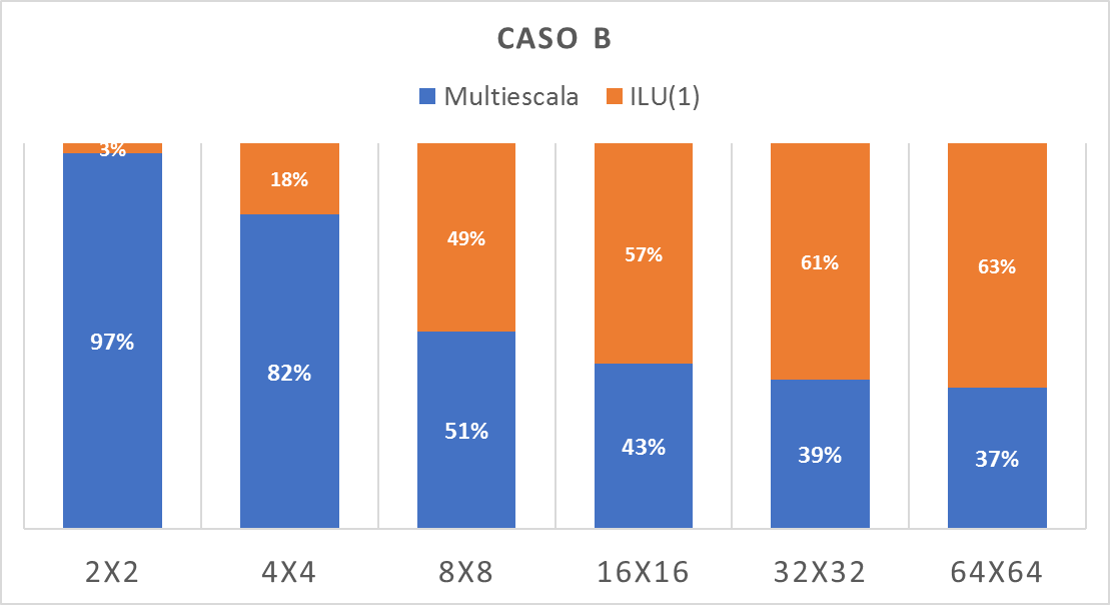
\includegraphics[width=0.45\textwidth]{chap08/figs/casoB_div.png}\label{fig:casoB_div}}
\qquad
\subfigure[ ]{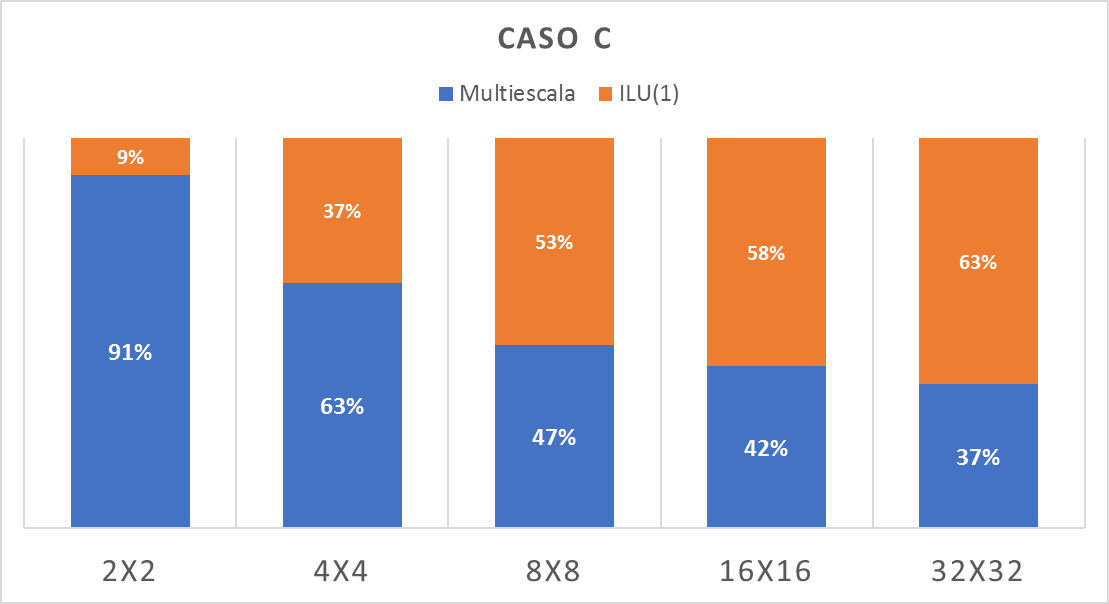
\includegraphics[width=0.45\textwidth]{chap08/figs/casoC_div.png}\label{fig:casoC_div}}
\subfigure[ ]{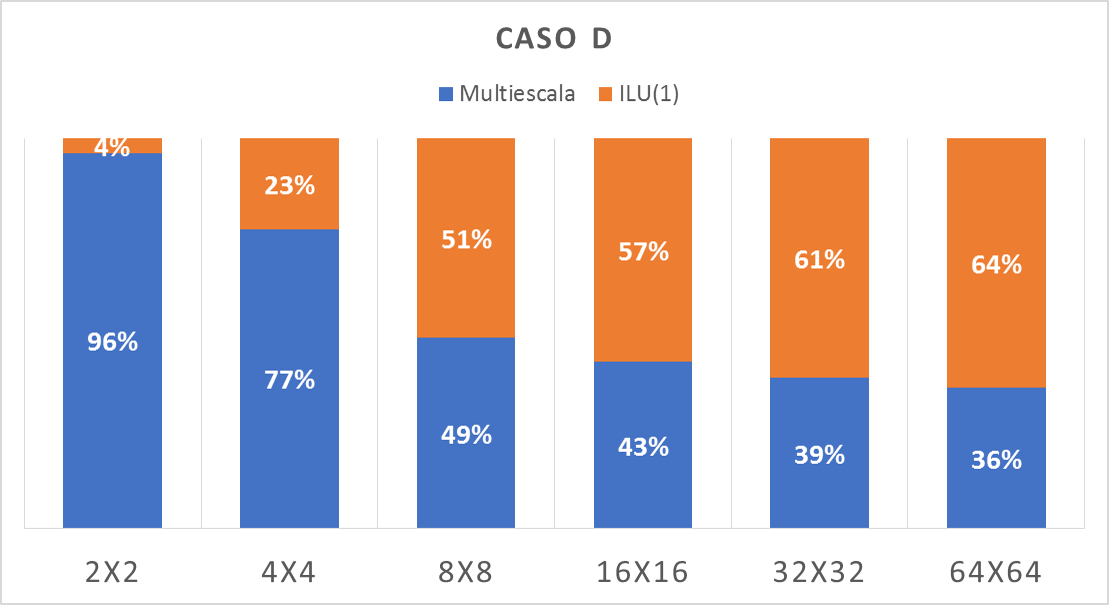
\includegraphics[width=0.45\textwidth]{chap08/figs/casoD_div.png}\label{fig:casoD_div}}
\qquad
\subfigure[ ]{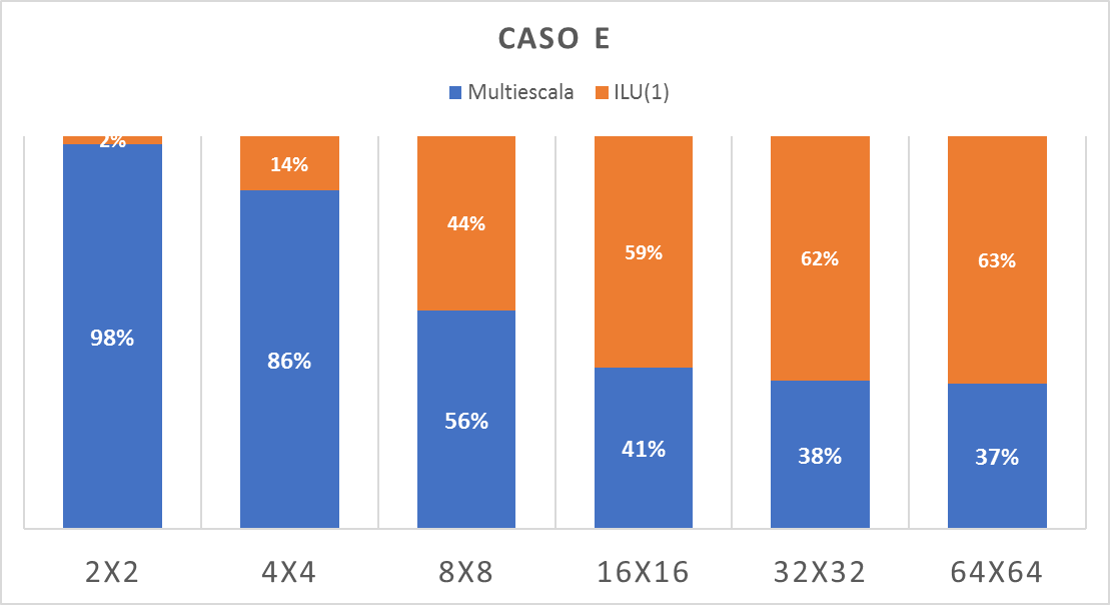
\includegraphics[width=0.45\textwidth]{chap08/figs/casoE_div.png}\label{fig:casoE_div}}
\caption{Proporção do tempo gasto entre ILU(1) e multiescala em pré-condicionador aditivo para o casos B, C, D e E.  }
\label{fig:proporcaoPrecondicionador}
\end{figure}


No caso B, a solução de menor tempo é quando o nível grosso é construído ao se montar elementos grossos utilizando 8x8 elementos finos. Ainda sobre o número de iterações, quando utilizado um elemento grosso de 2x2 o número de iterações é o menor encontrado, porém o custo de solução do sistema grosso impossibilita a utilização desse nível de engrossamento, uma maneira de aproveitar essa redução do número de iterações seria utilizar um pré-condicionador multiescala multinível conforme apresentado em \cite{multilevel} para volumes finitos, desse modo, não seria necessário resolver o sistema linear na malha 2x2 sendo necessário apenas aplicar uma relaxação nesse nível similarmente ao multigrid.

Na figura \ref{fig:reservatorio320x320_2} é apresentado a comparação da solução do sistema utilizando o melhor método multiescala com o gradiente conjugado utilizando como precondicionador o ILU(0), ILU(1) e solver multigrid Pyamg. É importante notar que há uma redução expressiva no número de iterações do Pyamg, e multiescala em relação aos ILU (redução em torno de 83\%) nos dois casos. Essa redução vem com o preço de um pré-condicionador com um custo computacional mais caro. Já uma comparação de tempo mostra uma redução de 72\% com MS(8,8)+ILU(1) em relação a execução com o pré-condicionador ILU(1). A comparação com o tempo do Pyamg pode não condizer com a realidade por se tratarem de implementações diferentes, posteriormente serão mostradas outros tipos de comparação com o Pyamg.

\begin{figure}[!htbp]
\centering
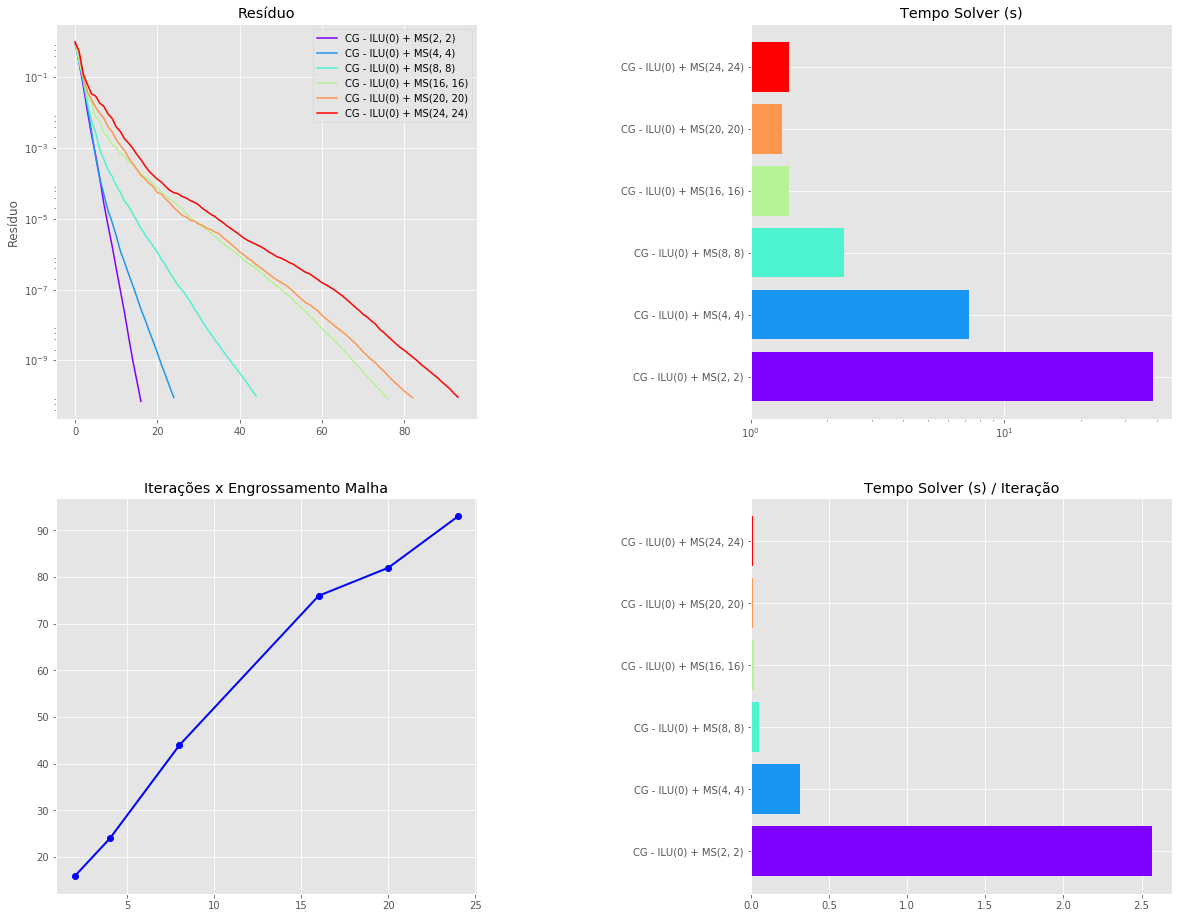
\includegraphics[width=\textwidth]{chap08/figs/reservatorio320x320_1.png}
\caption{Resultados para caso B. Histórico do resíduo relativo ao longo das iterações, tempo do solver em segundos, número de iterações e tempo do solver por iteração. }
\label{fig:reservatorio320x320_1} 
\end{figure}


\begin{figure}[!htbp]
\centering
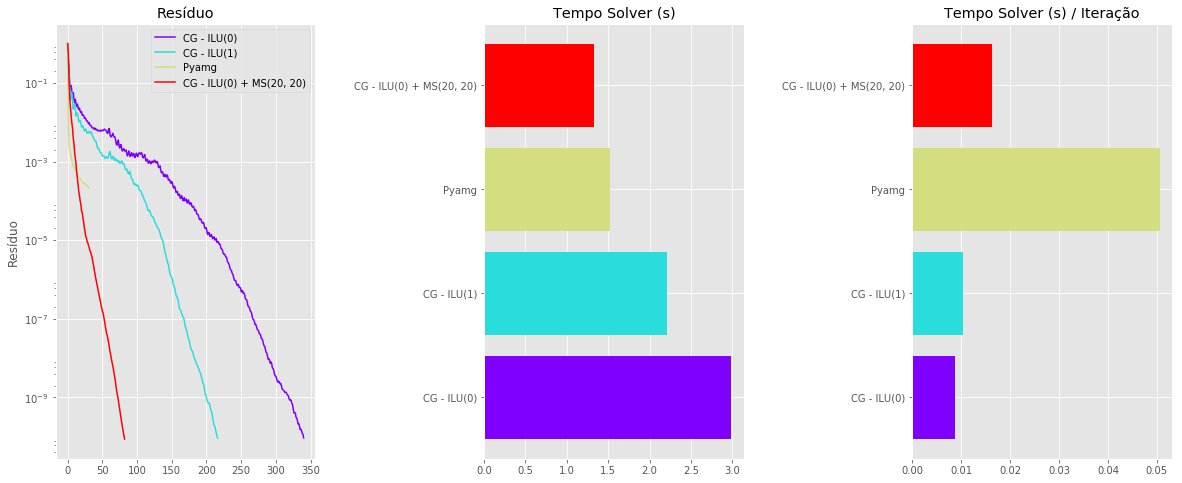
\includegraphics[width=\textwidth]{chap08/figs/reservatorio320x320_2.png}
\caption{Resultados para caso B. Histórico do resíduo relativo ao longo das iterações, tempo do solver em segundos e tempo do solver por iteração. }
\label{fig:reservatorio320x320_2}
\end{figure}


A seguir, as figuras \ref{fig:casoC_2}, \ref{fig:casoD_2} e \ref{fig:casoE_2} apresentam os resultados para os casos C, D e E. 
Em todos os gráficos é mostrado apenas o pré-condicionador multiescala que obteve o melhor desempenho entre os fatores de engrossamento de 2x2, 4x4, 8x8, 16x16, 32x32,  junto com os resultados do ILU(0), ILU(1) e Pyamg. Nos testes realizados o engrossamento da malha que teve o melhor desempenho de tempo foi o engrossamento 8x8.




\begin{figure}[h]
\center
\subfigure[Caso C ]{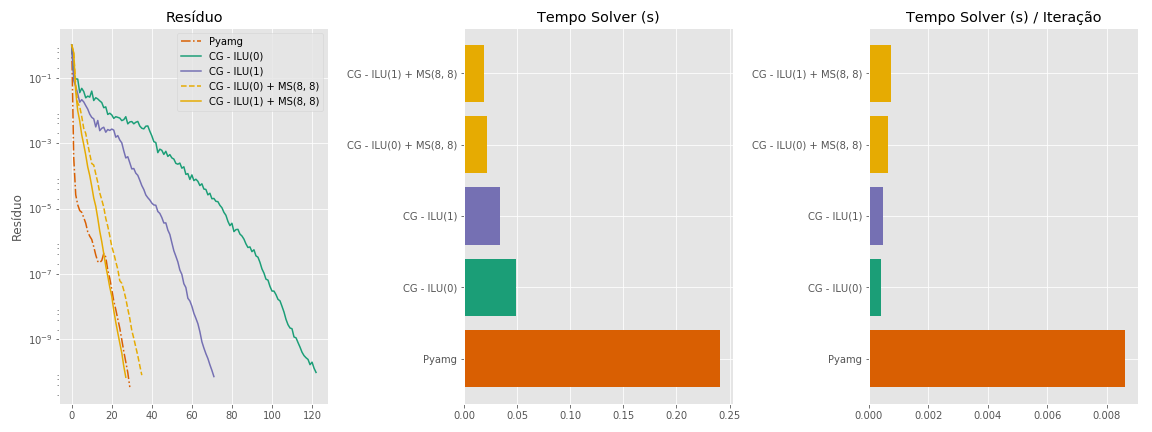
\includegraphics[width=\textwidth]{chap08/figs/casoC_2.png}\label{fig:casoC_2}}

\subfigure[Caso D ]{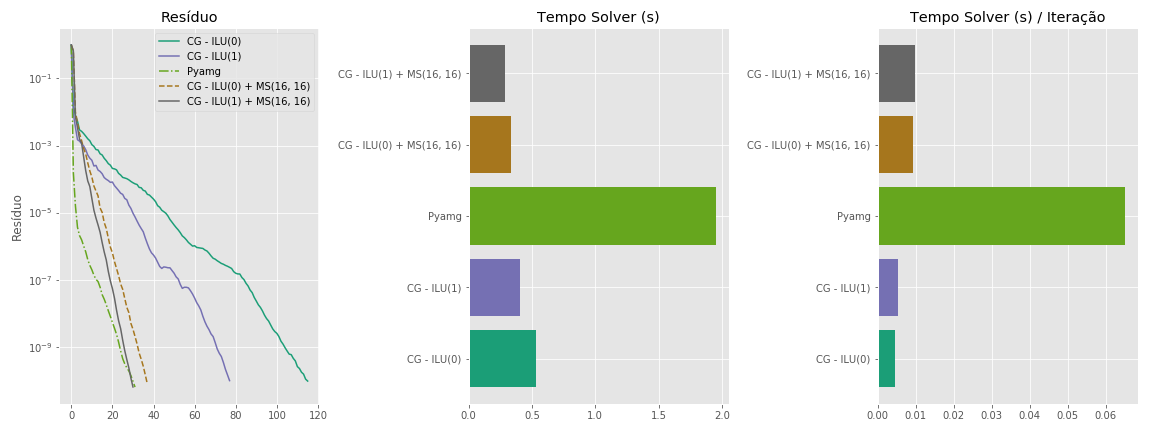
\includegraphics[width=\textwidth]{chap08/figs/casoD_2.png}\label{fig:casoD_2}}

\qquad
\subfigure[Caso E ]{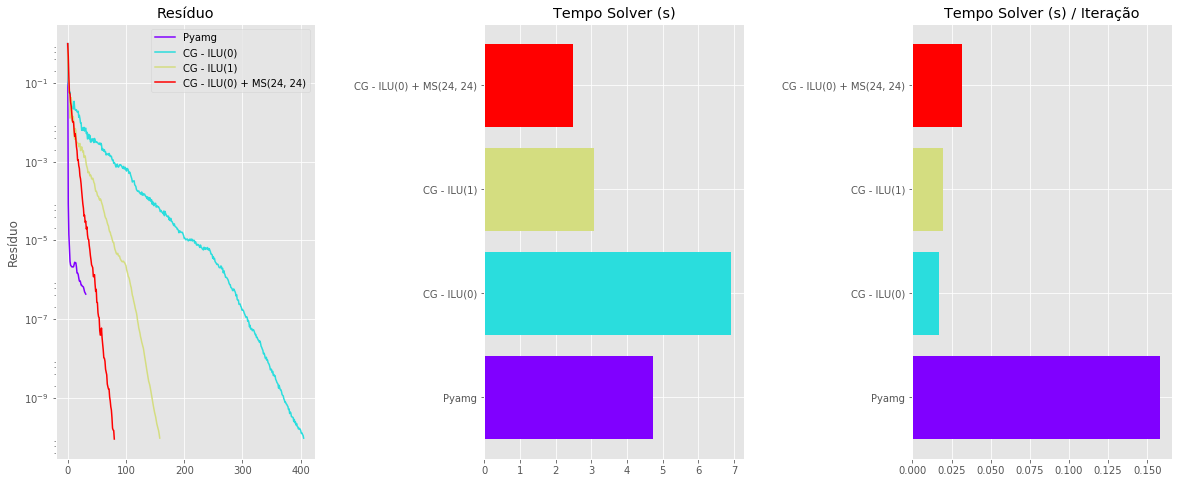
\includegraphics[width=\textwidth]{chap08/figs/casoE_2.png}\label{fig:casoE_2}}

\caption{ Histórico do resíduo, número de iterações e tempo do solver por iteração para caso C, D , E. O tempo é a media entre 10 rodadas. }

\label{fig:resultadosCDE}
\end{figure}

Nos casos C e D novamente a quantidade de iterações do Pyamg e multiescala foram semelhantes, mostrando um bom desempenho dos dois métodos, porém, no caso E o pré-condicionador multigrid começa decrescendo rapidamente mas passa por um ponto de resíduo $10^{-6}$ que a inclinação da queda muda rapidamente fazendo com que o solver multigrid tenha um número de iterações próxima ao do ILU(1). 


A Tabela $\ref{tab:comparacaoILU}$ apresenta a quantidade de iterações do solver, tempo e speed-up de cada caso do pré condicionador multiescala em relação ao ILU(1). Pode-se notar que os maiores speed-ups ocorreram nos casos com maiores dimensões (caso B e caso E) pois foram esses que obtiveram, proporcionalmente, as maiores reduções no número de iterações.

Em relação ao Pyamg, a Tabela \ref{tab:comparacaoMsxMgProlongamento} apresenta a quantidade de não zeros somando todos os níveis dos operadores de prolongamento do multigrid, o número de não zeros de todas as operações de prolongamento de um ciclo W e o número de não zeros do operador de prolongamento do multiescala. Nesse caso, pode-se constatar que a quantidade de não zeros dos operador de prolongamento do multiescala tem em torno de 2 a 2,2 vezes a quantidade de não zeros das multiplicações matriz vetor de um ciclo W do método multigrid sendo então uma vantagem do método multigrid.

Por outro lado, a Tabela \ref{tab:comparacaoMsxMgComplexidade} apresenta a complexidade dos operadores multigrid gerados para cada um dos casos. Além disso, possui a complexidade do ciclo W que considera as relaxações feitas em cada nível. Portanto, em relação as relaxações o multiescala necessita de bem menos capacidade computacional que fica em torno de 4,8 e 5,7 vezes menor que no multigrid que o torna mais eficiente nesse quesito. 
Assim, em relação ao caso E fica clara a vantagem do multiescala dado que o número de iterações realizadas foram 23 enquanto no multiescala foram 160 fazendo com o problema do prolongamento seja superado por ter feito menos que duas vezes a quantidade de iterações. Para os outros casos, há indícios de que o multiescala tenha se saído melhor dado que as operações de relaxação são bem mais custosas no multigrid.

\begin{table}[]

\caption{Tabela com comparação entre gradiente conjugado com pré-condicionador ILU(1) e pré-condicionador aditivo multiescala} \label{tab:comparacaoILU}

\begin{tabular}{c|c|c|c|c|c}
\cline{2-5}
                                    & \multicolumn{2}{c|}{\textbf{CG - ILU(1)}} & \multicolumn{2}{c|}{\textbf{CG - ILU(1) + MS(8, 8)}} &                                       \\ \hline
\multicolumn{1}{|c|}{\textbf{Caso}} & \textbf{Iterações}   & \textbf{Tempo(s)}  & \textbf{Iterações}          & \textbf{Tempo}         & \multicolumn{1}{c|}{\textbf{SpeedUp}} \\ \hline
\multicolumn{1}{|c|}{Caso B}        & 221                  & 2.224371           & 37                          & 0.608054               & \multicolumn{1}{c|}{3.66}             \\ \hline
\multicolumn{1}{|c|}{Caso C}        & 71                   & 0.034168           & 27                          & 0.018995               & \multicolumn{1}{c|}{1.80}             \\ \hline
\multicolumn{1}{|c|}{Caso D}        & 77                   & 0.334961           & 23                          & 0.148704               & \multicolumn{1}{c|}{2.25}             \\ \hline
\multicolumn{1}{|c|}{Caso E}        & 158                  & 3.082180           & 23                          & 0.803692               & \multicolumn{1}{c|}{3.84}             \\ \hline
\end{tabular}
\end{table}

%TODO fazer normalizado pelos não zeros da matriz
\begin{table}[]
\centering
\caption{Tabela com comparação entre número de não zeros das multiplicações matriz vetor de cada ciclo multigrid.} \label{tab:comparacaoMsxMgProlongamento}
\begin{tabular}{|c|c|c|c|c|}
\hline
\textbf{Caso} & \textbf{NNZ Mg} & \textbf{NNZ W} & \textbf{NNZ Ms} & \textbf{NNZ Ms/NNZ W} \\ \hline
Caso B        & 556916                       & 877595                   & 1799622                  & 2.05                                     \\ \hline
Caso C        & 29096                        & 42398                    & 92400                    & 2.18                                     \\ \hline
Caso D        & 205683                       & 355014                   & 705888                   & 1.99                                     \\ \hline
Caso E        & 1037150                      & 1718665                  & 3464370                  & 2.02                                     \\ \hline
\end{tabular}
\end{table}


\begin{table}[]
\centering
\caption{Tabela entre complexidade dos operadores multigrid e multiescala.} \label{tab:comparacaoMsxMgComplexidade}
\begin{tabular}{|c|c|c|c|}
\hline
\textbf{Caso} & \textbf{Complex. do Grid} & \textbf{Complex. do Ciclo} & \textbf{Complex. Multiescala} \\ \hline
Caso B        & 1.53                          & 5.18                           & 1.041                             \\ \hline
Caso C        & 1.57                          & 4.83                           & 1.033                             \\ \hline
Caso D        & 1.63                          & 6.53                           & 1.040                             \\ \hline
Caso E        & 1.55                          & 5.65                           & 1.041                             \\ \hline
\end{tabular}
\end{table}

\subsection{Acurácia da solução grossa}

Nos resultados mostrados na seção anterior, era utilizado um solver direto para resolver o sistema grosso. Em casos que a malha foi suficientemente reduzida esse tempo de solução é desprezível, porém, para casos o fator de engrossamento é pequeno resolver exatamente o nível grosso aumenta o tempo de execução (por exemplo, o caso ILU(1) + MS(2, 2) em \ref{fig:reservatorio320x320_1}). Além disso, caso modelos muito refinados sejam utilizados o espaço grosseiro possar ser grande o suficiente para resolver com métodos iterativos, como, por exemplo, para soluções de casos com centenas de milhões de elementos como os modelos mostrados em \cite{geomecrio}.

A Figura \ref{fig:toleranciaGrossa} apresenta a quantidade de iterações realizadas pelo gradiente conjugado com tolerância $10^{-10}$ no eixo y e a tolerância do solver do grid grosso no eixo. Para solução do grid grosso foi utilizado um gradiente conjugado pré-condicionador ILU(0). Pode-se constatar um aumento do número de iterações com o aumento da tolerância do solver grosso que era esperado. Mesmo com esse aumento o tempo de convergência total do processo melhora, podendo então, ser uma alternativa para casos em que os espaço grosso tenha dimensão elevada.



\begin{figure}[!htbp]
\centering
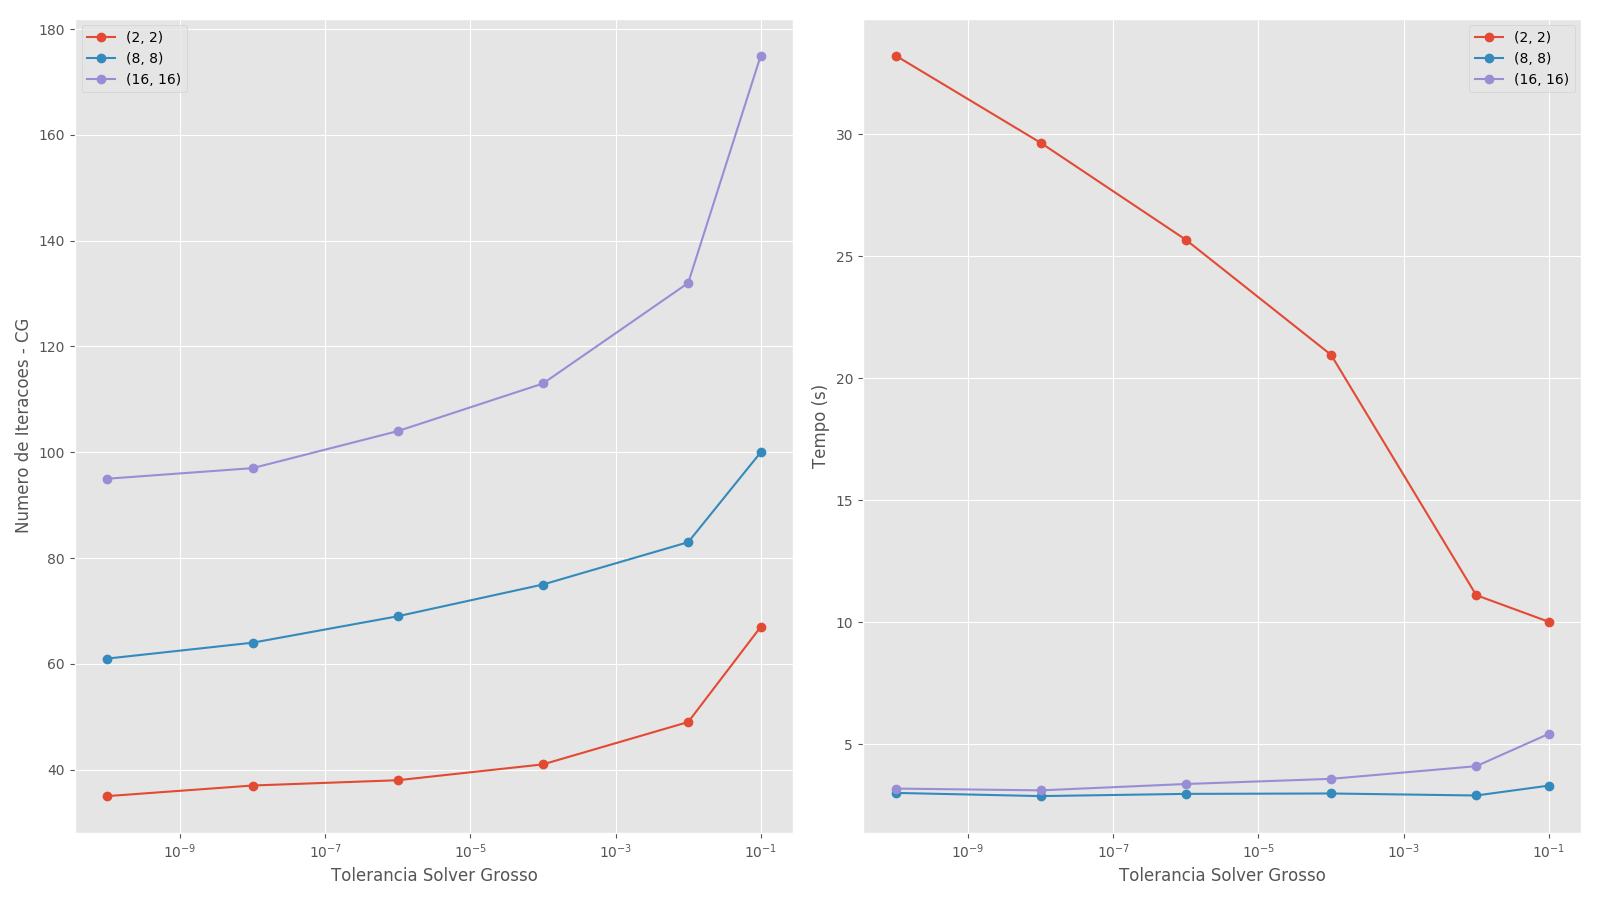
\includegraphics[width=\textwidth]{chap08/figs/Acuracia93MM.png}
\caption{ Variação do número de iterações do gradiente conjugado com tolerância do grid grosso para Caso E.}
\label{fig:toleranciaGrossa}
\end{figure}


